\chapter{Modular Scatter-Gather DMA}

\section{Avalon MM - Avalon MM}

\begin{table}[h]
    \centering
    \renewcommand{\arraystretch}{1.2}
    \begin{tabular}{|l|p{3cm}|p{3cm}|p{3cm}|}
    \hline
     & \textbf{Szerokość transferu: 32 bity} & \textbf{Szerokość transferu: 64 bity} & \textbf{Szerokość transferu: 128 bitów} \\ \hline
    \textbf{Zegar: 50MHz} & {191.06 MB/s} & {380.63 MB/s} & {720.01 MB/s} \\ \hline
    \textbf{Zegar: 100MHz} & {383.53 MB/s} & {715.43 MB/s} & {1452.71 MB/s} \\ \hline
    \textbf{Zegar: 200MHz} & {724.94 MB/s} & {1480.24 MB/s}  & {2390.95 MB/s} \\ \hline
    \end{tabular}
    \caption{Przepustowość transferu DMA w zależności od częstotliwości zegara i szerokości transferu}
    \label{tab:mm_mm}
\end{table}

\begin{figure}[h]
    \centering
    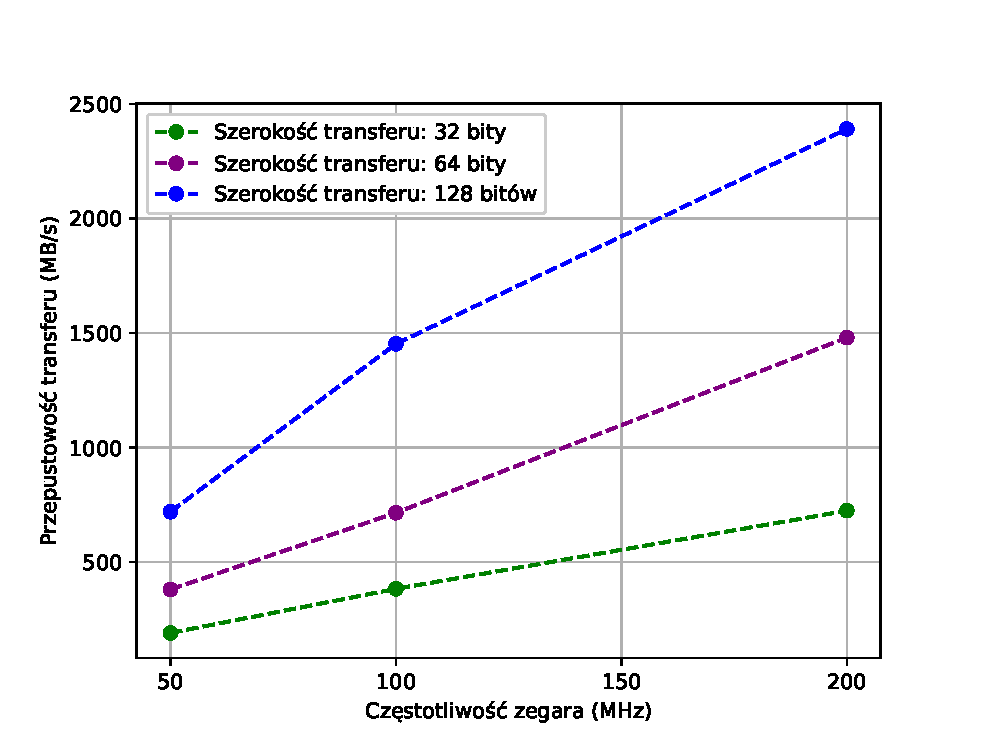
\includegraphics[width=0.7\textwidth]{mm_mm.eps}
    \caption{Zależność prędkości transferu od częstotliwości zegara}
    \label{fig:mm_mm}
\end{figure}

\section{Avalon MM - Avalon ST - Avalon MM}

\begin{table}[h]
    \centering
    \renewcommand{\arraystretch}{1.2}
    \begin{tabular}{|l|p{3cm}|p{3cm}|p{3cm}|}
    \hline
    \diagbox[height=1.7cm, width=4.8cm]{\bfseries{\small Częstotliwość zegara}}{\bfseries{\small Szerokość transferu}}
    & \textbf{32 bity} & \textbf{64 bity} & \textbf{128 bitów} \\ \hline
    \textbf{\hspace{1.6cm}50 MHz} & {188.12 MB/s} & {375.75 MB/s} & {696.90 MB/s} \\ \hline
    \textbf{\hspace{1.6cm}100 MHz} & {379.88 MB/s} & {698.40 MB/s} & {1424.82 MB/s} \\ \hline
    \textbf{\hspace{1.6cm}200MHz} & {707.35 MB/s} & {1442.78 MB/s} & {2350.05 MB/s} \\ \hline
    \end{tabular}
    \caption{Przepustowość transferu DMA w zależności od częstotliwości zegara i szerokości transferu}
    \label{tab:mm_st_mm}
\end{table}

\begin{figure}[h]
    \centering
    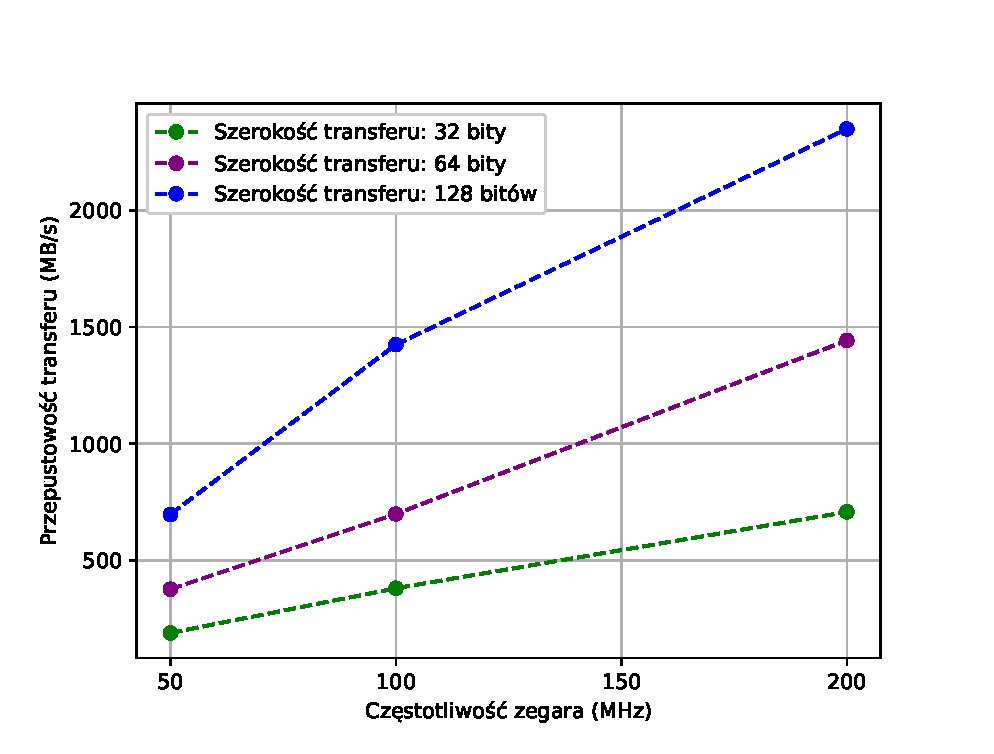
\includegraphics[width=0.7\textwidth]{mm_st.eps}
    \caption{Zależność prędkości transferu od częstotliwości zegara}
    \label{fig:mm_st}
\end{figure}